\chapter{Konzeption}
\label{chapter-konzept}

In diesem Kapitel wird die eigentliche Erkenntnis der Arbeit beschrieben. Die eingangs beschriebenen
Anforderungen definieren, was das System zu leisten hat. Im Folgenden werden die Funktionalitäten
definiert, um zu beschreiben, wie das System die Anforderungen gewährleisten kann. Des Weiteren wird
auf die Wahl der Frameworks und darauffolgend auf die Systemarchitektur eingegangen.

\section{Funktionalität}
\label{section:funktionalitaeten}
Im Folgenden werden die für das System relevanten Funktionalitäten aufgeführt. Zur besseren
Lesbarkeit wurden die Funktionalitäten nach Benutzergruppen aufgeteilt.

\subsection{Funktionalitäten für (B)eide}
Zu Beginn werden Funktionalitäten, welche für Verleihende und Ausleihende von Bedeutung sind
näher erläutert (\ref{table:ft-b}).

\begin{table}[h]
    \centering
    \caption{Funktionalitäten für (B)eide}
    \begin{longtable}{lll}
        \arrayrulecolor{maincolor}\hline
        \sffamily\color{maincolor}ID & \sffamily\color{maincolor}Titel    &
        \sffamily\color{maincolor}Anforderungen \\
        \arrayrulecolor{maincolor}\hline
        Ft-B-1                       & Authentifizierung über LDAP  & \anfref{F70} \anfref{F80} \\
        Ft-B-2                       & Übersicht über ausleihbare Assets  & \anfref{V20}
        \anfref{Z20} \anfref{F50} \anfref{K10} \anfref{F10} \anfref{F30} \\
        Ft-B-3                       & Verfügbarkeit von Assets           & \anfref{V20}
        \anfref{Z20} \anfref{F50} \anfref{K10} \anfref{F10} \anfref{F30} \\
        Ft-B-4                       & Zuständigkeitsbereich              & \anfref{F50} \\
        Ft-B-5                       & Benachrichtigungen \& Erinnerungen & \anfref{F100}
        \anfref{F110} \anfref{F120}                                     \\
        Ft-B-6                       & Material-Suche                     & \anfref{V20}
        \anfref{Z20} \anfref{K10} \anfref{F10} \anfref{F30} \\
        Ft-B-7                       & Filtern und Sortieren              & \anfref{V30}
        \anfref{F30} \anfref{F70}                                        \\
        Ft-B-8                       & Detailansicht                      & \anfref{V50}
        \anfref{Z30} \anfref{F40} \anfref{F50}                           \\
        \arrayrulecolor{maincolor}\hline
    \end{longtable}
    \label{table:ft-b}
\end{table}

{\sffamily\color{maincolor}{Ft-B-1 | Authentifizierung über LDAP}}\\
Mithilfe der Verknüpfung zum LDAP der Universität zu Lübeck, können sich Nutzende mit einem bereits
existierenden IDM Account einloggen. Folglich muss kein neues Konto erstellt werden. Außerdem kann
überprüft werden, ob es sich bei der Anmeldung um Studierenden oder \ac{wimi} handelt und die damit
einhergehenden Authentifizierung prüfen. Des Weiteren verhindert die Nutzung von LDAP das Eindringen
unbefugter Personen. 


    {\sffamily\color{maincolor}{Ft-B-2 | Übersicht über ausleihbare Assets }}\\
Die Übersicht, der am \ac{imis} vorhandenen Assets, wurde mittels Kategorien umgesetzt. Dafür gibt es
eine Übersicht, bei der alle Assets eingesehen werden können. Die einzelnen Kategorien beinhalten
Unterkategorien. In der Übersicht werden Informationen, wie Name, Seriennummer, Marke und Status
eines Assets angezeigt.

    {\sffamily\color{maincolor}{Ft-B-3 |  Verfügbarkeit von Assets }}\\
Der Status eines Asset \textit{(Verfügbar, Nicht verfügbar, Hinweis)} muss klar ersichtlich sein.
Dies geschieht mittels Color-Coding.  


{\sffamily\color{maincolor}{Ft-B-4 | Zuständigkeitsbereich }}\\
Um für Ausleihende Kontaktinformationen anzeigen zu können \textit{(Ft-A-6)}, müssen die
Zuständigkeitsbereiche eingetragen werden können. Außerdem sollten alternative Ansprechpartner:innen
kenntlich gemacht werden, um Abholtermine aufgrund von Krankheit oder Homeoffice nicht verschieben
zu müssen. Für Rückfragen zu einem Asset sind Kontaktinformation zu Ansprechpartner:innen
(Verleihende) sowie E-Mail-Adressen hinterlegt.

{\sffamily\color{maincolor}{Ft-B-5 | Benachrichtigungen \& Erinnerungen }}\\
Verleihende werden nach dem Abschluss eines von ihnen verantwortlichen Assets benachrichtigt. Die
Benachrichtigung umfasst Informationen, wer das Asset, wann reserviert hat und wann die Abholung für
das Asset stattfinden soll. Außerdem wird es eine direkte Weiterleitungsmöglichkeit geben, sollten
Verleihenden nicht können. Nachdem die Reservierung eines Assets stattgefunden hat, erhalten
Ausleihende eine Zusammenfassung über die Ausleihdaten und einen Hinweis, wann die Abholung
stattfindet. Außerdem werden Kontaktinformation des Verleihenden angezeigt (Name, E-Mail und
Lagerort des Assets). Zusätzlich erhalten Verleihende und Ausleihende eine Erinnerung, sobald die
Abholung oder Rückgabe eines Assets ansteht.


    {\sffamily\color{maincolor}{Ft-B-6 | Material-Suche }}\\
Die Material-Suche dient zum einen einer simplen aber unterstützenden Kategorieneinteilung, zum
anderen für das gezielte Suchen nach Verfügbarkeiten (verfügbar, Nicht verfügbar und Hinweis). Das
gezielte Suchen nach Verfügbarkeit wird durch die Aufforderung den Ausleihzeitraum anzugeben
ermöglicht. Daraufhin gibt es die Möglichkeit gewünschte Materialien in einem Suchfeld einzugeben
oder über die Kategorien nach dem Asset zu suchen. Das Suchefeld gibt bereits beim eintippen
Vorschläge. Die Vorschläge umfassen Assets direkt oder Kategorien. Bei mehreren Assets werden
mithilfe einer Aufzählung alle Elemente angezeigt, die bereits für eine Reservierung ausgewählt
wurden.

    {\sffamily\color{maincolor}{Ft-B-7 | Filtern und Sortieren }}\\
Um das Finden für Assets leichter zu gestalten sollen Nutzende stets nach Kategorie, Nutzen und
Verfügbarkeit filtern können. Außerdem ist das Sortieren von A-Z oder Z-A möglich. Um bei der
Anzeige einen Überblick über die Menge der Assets behalten zu können wir die Anzahl der Assets in
der ausgewählten Kategorie angezeigt.

{\sffamily\color{maincolor}{Ft-B-8 | Detailansicht }}\\
In der Detailansicht werden die Assets und deren Eigenschaften dargestellt. Hierbei werden
Informationen wie: Name, Seriennummer, Artikelbeschreibung, technische Details und
Kontaktinformation der Verleihenden dargestellt. Des Weiteren kann der Ausleihzeitraum eingestellt
und eingesehen werden, wann ein Asset verfügbar ist. In Form eines Button wird sichtbar, dass das
Asset zur Ausleihe hinzugefügt werden kann. Das hinzufügen wird durch eine Pop-Up-Mitteilung
bestätigt.


\subsection{Funktionalitäten für Verleihende}
Im Folgenden werden Funktionalitäten, welche für Verleihende von Bedeutung sind näher erläutert
(\ref{table:ft-v}).

\begin{table}[h]
    \centering
    \caption{Funktionalitäten für (V)erleihenden }
    \begin{longtable}{lll}
        \arrayrulecolor{maincolor}\hline
        \sffamily\color{maincolor}ID & \sffamily\color{maincolor}Titel &
        \sffamily\color{maincolor}Anforderungen \\
        \arrayrulecolor{maincolor}\hline
        Ft-V-1                       & Dashboard               & ??? \\
        Ft-V-2                       & Bearbeiten des Assetstatus      & \anfref{F150} \\
        Ft-B-4                       & Kalenderansicht   für Verleihende                 &
        \anfref{V50} \anfref{Z30} \anfref{F40} \anfref{F50}                           \\
        Ft-V-3                       & Pflege von Assets               & \anfref{F130} \\
        Ft-V-4                       & Pflege der Datenbank            & \anfref{F140} \\
        \arrayrulecolor{maincolor}\hline
    \end{longtable}
    \label{table:ft-v}
\end{table}

{\sffamily\color{maincolor}{Ft-V-1 | Dashboard }}\\
Die Dashboard-Ansicht umfasst eine Aufgabenliste des ausgewählten Tages. Die Aufgaben umfassen
Abholungs- oder Rückgabeterminen sowie Wartungserinnerungen. Durch einer Wochenliste kann zwischen
den Tagen gewechselt werden. Außerdem werden die aktuellsten Benachrichtigungen angezeigt.



{\sffamily\color{maincolor}{Ft-V-2 | Bearbeiten des Assetstatus }}\\
Assets, welche an Ausleihende übergeben wurde, müssen zunächst manuell in ihrem Status bestätigt
werden. Hierfür ist eine simple Funktion vorgesehen, sodass der Status des Assets schnell aktuell
gehalten werden kann. Außerdem soll das System, nachdem eine Abholung oder Rückgabe stattgefunden
hat, eine Benachrichtigung an Verleihende senden, sollte der Status nicht bereits bestätigt worden
sein.

{\sffamily\color{maincolor}{Ft-B-4 | Kalenderansicht für Verleihende}}\\
Die Kalenderansicht für Verleihende beinhaltet eine Übersicht, über alle Assets, welche gerade
Verliehen sind. Mithilfe einer Monatsübersicht werden Termin zur Asset-Abholung, Rückgabe oder zur
Wartung angezeigt. In einer Wochenansicht auf dem Dashboard gibt es eine detailreichere Ansicht
eines jeweiligen Tages.


    {\sffamily\color{maincolor}{Ft-V-3 | Pflege von Assets   }}\\
    \todo[]{baue ich eigentlich nict mit ein}
Mit Hilfe der Zuständigkeitsbereich \textit{(Ft-V-2)} kann die Pflege der Assets besser kontrolliert
werden. Außerdem können durch Erinnerungen und Checkliste Wartungen weniger leicht vergessen werden
und besser aufgeteilt werden.


    {\sffamily\color{maincolor}{Ft-V-4 | Pflege der Datenbank }}\\
    \todo[]{Läuft über Snipe-IT}
Das Prinzip des Reservierungstools kann nur funktionieren, wenn Neuanschaffung in die Datenbank
eingepflegt werden. Hierfür soll eine Anleitung für Verleihende sichtbar gemacht werden. Wichtig
hierbei ist, dass das Eintragen nicht nur für das Ausleihen hilfreich ist, sondern auch für eine
generelle Übersicht des Bestands am \ac{imis}.

\subsection{Funktionalitäten für (A)usleihende}
Im Folgenden werden Funktionalitäten, welche für Ausleihenden von Bedeutung sind näher erläutert
(\ref{table:ft-A}).

\begin{table}[h]
    \centering
    \caption{Funktionalitäten für (A)usleihende }
    \begin{longtable}{lll}
        \arrayrulecolor{maincolor}\hline
        \sffamily\color{maincolor}ID & \sffamily\color{maincolor}Titel &
        \sffamily\color{maincolor}Anforderungen \\
        \arrayrulecolor{maincolor}\hline
        Ft-A-1                       & Startübersicht                  & \anfref{F60} \\
        Ft-A-2                       & Reservierungs-Checkout          & \anfref{F60} \anfref{F150}
        \\

        Ft-A-3                       & Rückgabe-Checkliste             & ??? \\
        Ft-B-4                       & Kalenderansicht für Ausleihende                  &
        \anfref{V50} \anfref{Z30} \anfref{F40} \anfref{F50}                           \\
        \arrayrulecolor{maincolor}\hline
    \end{longtable}
    \label{table:ft-A}
\end{table}


{\sffamily\color{maincolor}{Ft-A-1 | Startübersicht }}\\
Die Startseite soll Nutzenden helfen, einen Überblick zu erlangen. Für Erstnutzende, sind Hinweise
für die Materal-Suche  in Form von Button gegeben. Für Nutzende, die bereits Assets ausgeliehen
haben, wird eine Übersicht über Laufende, Kommende und Vergangene Reservierungen angezeigt. Wichtige
Informationen, wie der Zeitraum werden direkt auf einen Blick ersichtlich.

    {\sffamily\color{maincolor}{Ft-A-2 | Reservierungs-Checkout }}\\
Mithilfe des Reservierungs-Checkouts können alle ausgewählten Assets im Überblick eingesehen werden.
Außerdem werden alle Ausleihdaten, wie Zeitraum der Ausleihe, Abholung und Rückgabe aufgeführt. Des
Weiteren gibt es die Möglichkeit, alle Ausleihdaten bearbeiten zu können, sollte ein Datum oder eine
Uhrzeit unpassend sein. Abschließend werden die Regeln und Sicherheitshinweise aufgeführt. Mithilfe
einer AGB Bla erklärung, gilt die Reservierungstools als vertraglich abgeschlossen.

    {\sffamily\color{maincolor}{Ft-A-3 | Rückgabe-Checkliste}}\\
Bevor die ausgeliehenen Assets an Verleihende zurückgeben werden, wird eine Checkliste für das
jeweilige Asset angezeigt, bei der Hinweise stehen wie: SD-Karte geleert, Assets auf
Ursprungseinstellungen zurückgestellt, Akkus geladen. Diese Funktionalität soll insbesondere dafür
sorgen, dass nachfolgende Ausleihende Assets direkt nutzen können.

{\sffamily\color{maincolor}{Ft-B-4 | Kalenderansicht für Ausleihende}}\\
\todo[]{Mehr arbeit.. eher raus nehmen?}
Die Kalenderansicht für Ausleihende beinhaltet eine Übersicht, über alle Assets, welche gerade
ausgeliehen sind. Mithilfe einer Monatsübersicht werden Termin zur Asset-Abholung oder Rückgabe
angezeigt. 

%Frameworks
\section{Frameworks}
\label{section:frameworks}
Die Frameworkwahl nimmt, durch die unterschiedlichen Arbeitsweisen und Funktionen der Frameworks,
enormen Einfluss auf den Entwurf eines Systems und wird daher im Folgenden näher erläutert. Zunächst
wird auf die Anforderungen der vorliegenden Arbeit und die damit einhergehenden relevanten
Anforderungen an die Frameworks eingegangen. Resultierend daraus, werden die nutzenden Frameworks
definiert.

\subsection{Relevante Anforderung an ein Framework}
\todo[inline]{Ausführlicher?}
Die Grundlage der Auswahl, der im Rahmen dieser Arbeit eingesetzten Frameworks, bilden die eingangs
beschriebenen Anforderungen (\ref{section:anforderung}). Dem System wird vorausgesetzt, dass es sich
um eine Web-Anwendung mit Fokus auf den Einsatz im mobilen Kontext (\anfref{R10}\anfref{R40}). Für
Nutzende ist es wichtig, dass das System dauerhaft erreichbar ist (\anfref{R50}). Aus funktionaler
Sicht müssen die Frameworks eine Unterstützung für progressive Web-Applikationen bieten. Folglich
ist auch eine Unterstützung für HTTPS notwendig (\anfref{Q50}). Außerdem sollte es einfache
Möglichkeiten zur Verknüpfung von LDAP bieten (\anfref{K10} \anfref{F90}).

\subsection{Wahl der genutzten Frameworks}
Aufbauend auf den Anforderungen und der am \ac{imis} bereits eingesetzten Asset Managementsoftware
\textit{Snipe-IT} werden im Folgenden die gewählten Frameworks erläutert.

\subsubsection{Asset Managementsoftware Snipe-IT}
\todo[inline]{Referenzierungen hinzufügen}

Die Basis für das in dieser Arbeit umgesetzte System schafft die Asset Managementsoftware
\textit{Snipe-IT} \cite{noauthor_home_nodate}, welche bereits am \ac{imis} eingesetzt wird.
\textit{Snipe-IT} ist eine kostenlose, quelloffene IT-Asset-Verwaltungs-Plattform, welche das
Nachverfolgen von Software-Lizenzen, Hardware und Verbrauchsgegenständen ermöglicht. Genannte Assets
können über ein Dashboard hinzugefügt, verwaltet und gelöscht werden. Über Labels können Assets zur
Übersichtlichkeit in verschiedene Kategorien eingeordnet werden, während Tags ein Asset eindeutig
identifizieren (z. B. Seriennummer). Zudem ermöglicht das „Checkin/Checkout“-System die
Nachverfolgung aller Assets, falls diese zum Beispiel an Person ausgeliehen werden. Zu jedem
Zeitpunkt kann ein Asset maximal einer Person zugeordnet werden, wodurch das mehrfache gleichzeitige
Ausleihen eines Assets verhindert wird. Darüber hinaus beschreiben Status-Label den Zustands eines
Assets und ob dieses ausgeliehen werden kann. Alle Funktionalitäten können zudem über eine REST-API
programmatisch genutzt werden. Des Weiteren verfügt \textit{Snipe-It} über eine Schnittstelle,
welche die Integration von LDAP stark vereinfacht.

\subsubsection{Reservierungsinterface}
Das Reservierungsinterface wird mit Fastify\footnote{\url{https://www.fastify.io/}},
Prisma\footnote{\url{https://www.prisma.io/}} und
PostgreSQL\footnote{\url{https://www.postgresql.org/}} umgesetzt. 

\subsubsection{Vue.js}
Für Grundlage des Frontends wird Vue.js\footnote{\url{https://vuejs.org/}} verwendet. Vue.js ist
eine progressive JavaScript Framework. Bei der Nutzung von Vue
CLI\footnote{\url{https://cli.vuejs.org/}} kann eine PWA-Funktionalität mithilfe des
\inlinecode{@vue/cli- plugin-pwa}-Pakets schnell eingebunden werden. Zudem steigt das Framework in
der Zufriedenheit und Verwendung laut \citeA{noauthor_state} im Vergleich zu Angular über die Jahre
stetig an (\ref{fig:vue}). Außerdem zeigt Vue.js in den Leistungs-Benchmarks positive Merkmale
\todo[]{(Krause, 2022)}. Zusätzlich zu den bereits aufgeführten Eigenschaften wird Vue.js aufgrund der
begrenzten Implementierungszeit und bestehende Erfahrung gewählt.

\begin{figure}[h]
    \centering
    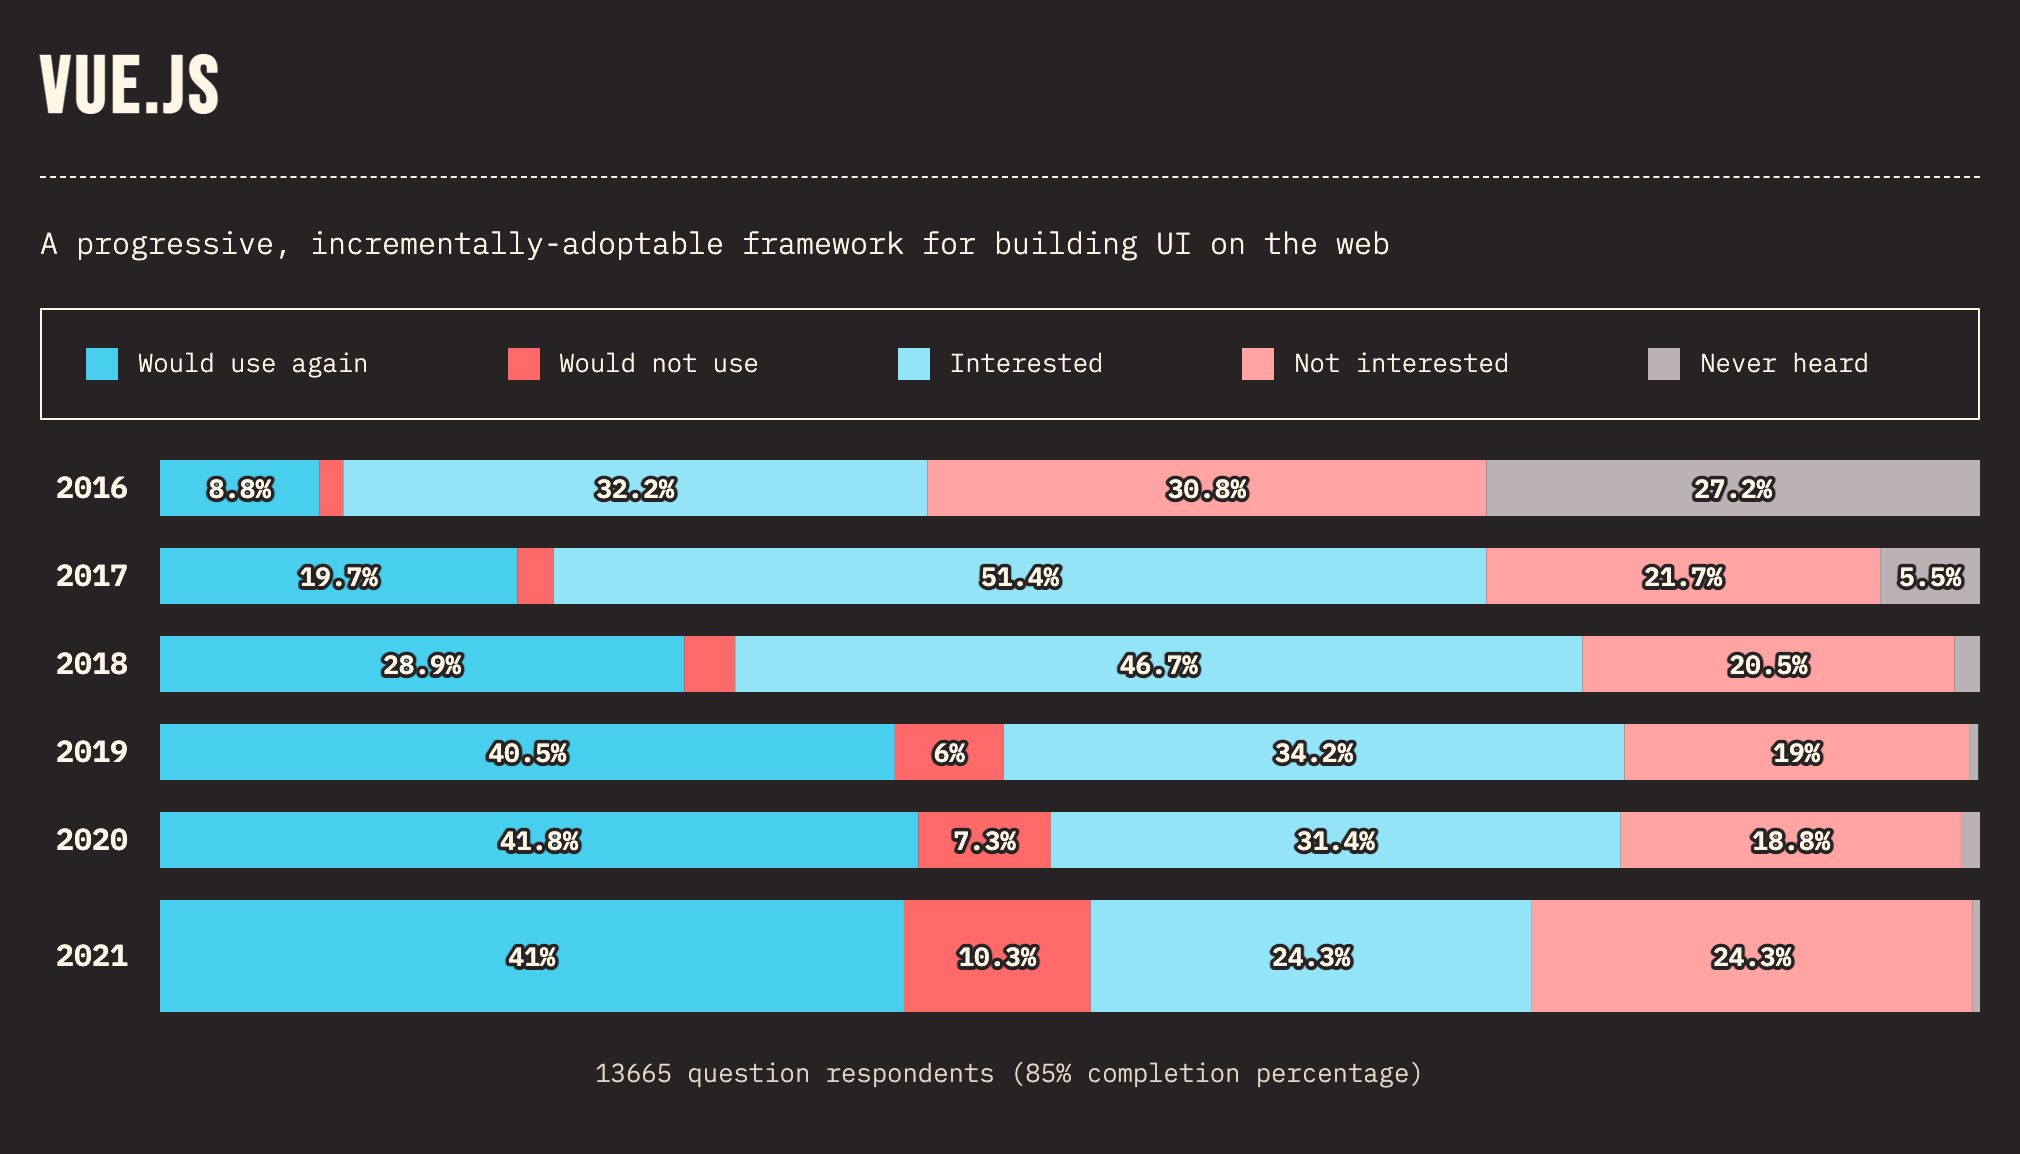
\includegraphics[scale=0.22]{Bilder/vuejs.png}
    \caption[Vue.js A progressive, incrementally-adoptable framework for building UI on the web]{Vue.js - A progressive, incrementally-adoptable framework for building UI on the web}
    \label{fig:vue}
\end{figure}


\section{Systemarchitektur}
Mithilfe der bereits festgelegten Frameworks (\ref{section:frameworks}) wurde die Systemarchitektur
entwickelt. Die Systemarchitektur gibt eine Übersicht über die technische Umsetzung des Systems,
welches im Wesentlichen aus den folgenden drei Komponenten besteht (\ref{fig:uml}): dem Snipe-IT
Server, dem Reservierungsinterface und dem Front-End, welches mit Vue.js realisiert wurde.

\subsection{Snipe-IT}
Die Datenbank und API von Snipe-IT bilden die Ausgangsposition des Systems. Folglich wird das
Verwalten der Assets selbst, was am \ac{imis} vorhanden ist und alle Eigenschaften zu den Assets
über Snipe-IT stattfinden und gespeichert. Über die bereitgestellte API werden die gespeicherten
Daten für alle weiteren Komponenten bereitgestellt. Durch die eingeschränkten Funktionen der
Kalender-Funktion und die fehlende Möglichkeit Termine in der Zukunft auswählen zu können, wird das
Reservierungsinterface benötigt.

\subsection{Reservierungsinterface}
Das Reservierungsinterface nutzt die von Snipe-IT bereitgestellten Daten. Die Hauptaufgabe der
Schnittstelle ist das Reservieren von Assets in die Zukunft. Das Back-End wird mit Fastify, Prisma
und PostgreSQLumgesetzt. Fastify ist ein Webserver-Framework, welcher das Routing erleichtert.
Prisma ist ein ORM (Object-Relational-Mapper) welches die Nutzung der PostgreSQL-Datenbank im
Webserver erleichtert. Die Weboberfläche läuft über die Web-App, hierbei wird mithilfe der LDAP
Authentifizierung die jeweilige Ansicht bestimmt.

\subsection{Web-App}
Über die Web-App bildet die Oberfläche für Ausleihende und ermöglicht es die Assets einsehen zu
können, zu suchen, zu buchen. Außerdem laufen über die Web-Oberfläche alle administrativen Aufgaben
für Verleihende, wie das Aktualisieren eines Assetstatus. Folglich greift die Web-App ebenso wie die
anderen Komponenten auf Snipe-IT zu, um die Assetinformationen anzeigen zu können. 

Beim Server-Rendering-Ansatz muss die Seite für jeden Aufruf neu generiert. Daher wird die Web-App
separat von Snipe-IT bereitgestellt und statisch gehostet. Das Generieren der Web-App findet somit
nur einmalig statt.

\subsection{Interaktion der Komponenten}
Um ein besseres Verständnis der Interaktion von einzelnen Komponenten voraussetzen zu können wurde
ein UML-Sequenzdiagramm erstellt (\ref{fig:uml}). Bei der vierten Komponente handelt es sich um das
LDAP der Universität zu Lübeck. Mithilfe der Integration können Nutzende sich mit dem bereits
bestehenden IDM Account anmelden. Zum einen kann somit sichergestellt werden, dass nur befugte
Personen Assets einsehen und ausleihen können. Zum anderen erleichtert es den Nutzenden den
Ausleihprozess, da kein neuer Account erstellt werden muss.

\begin{figure}[h]
    \centering
    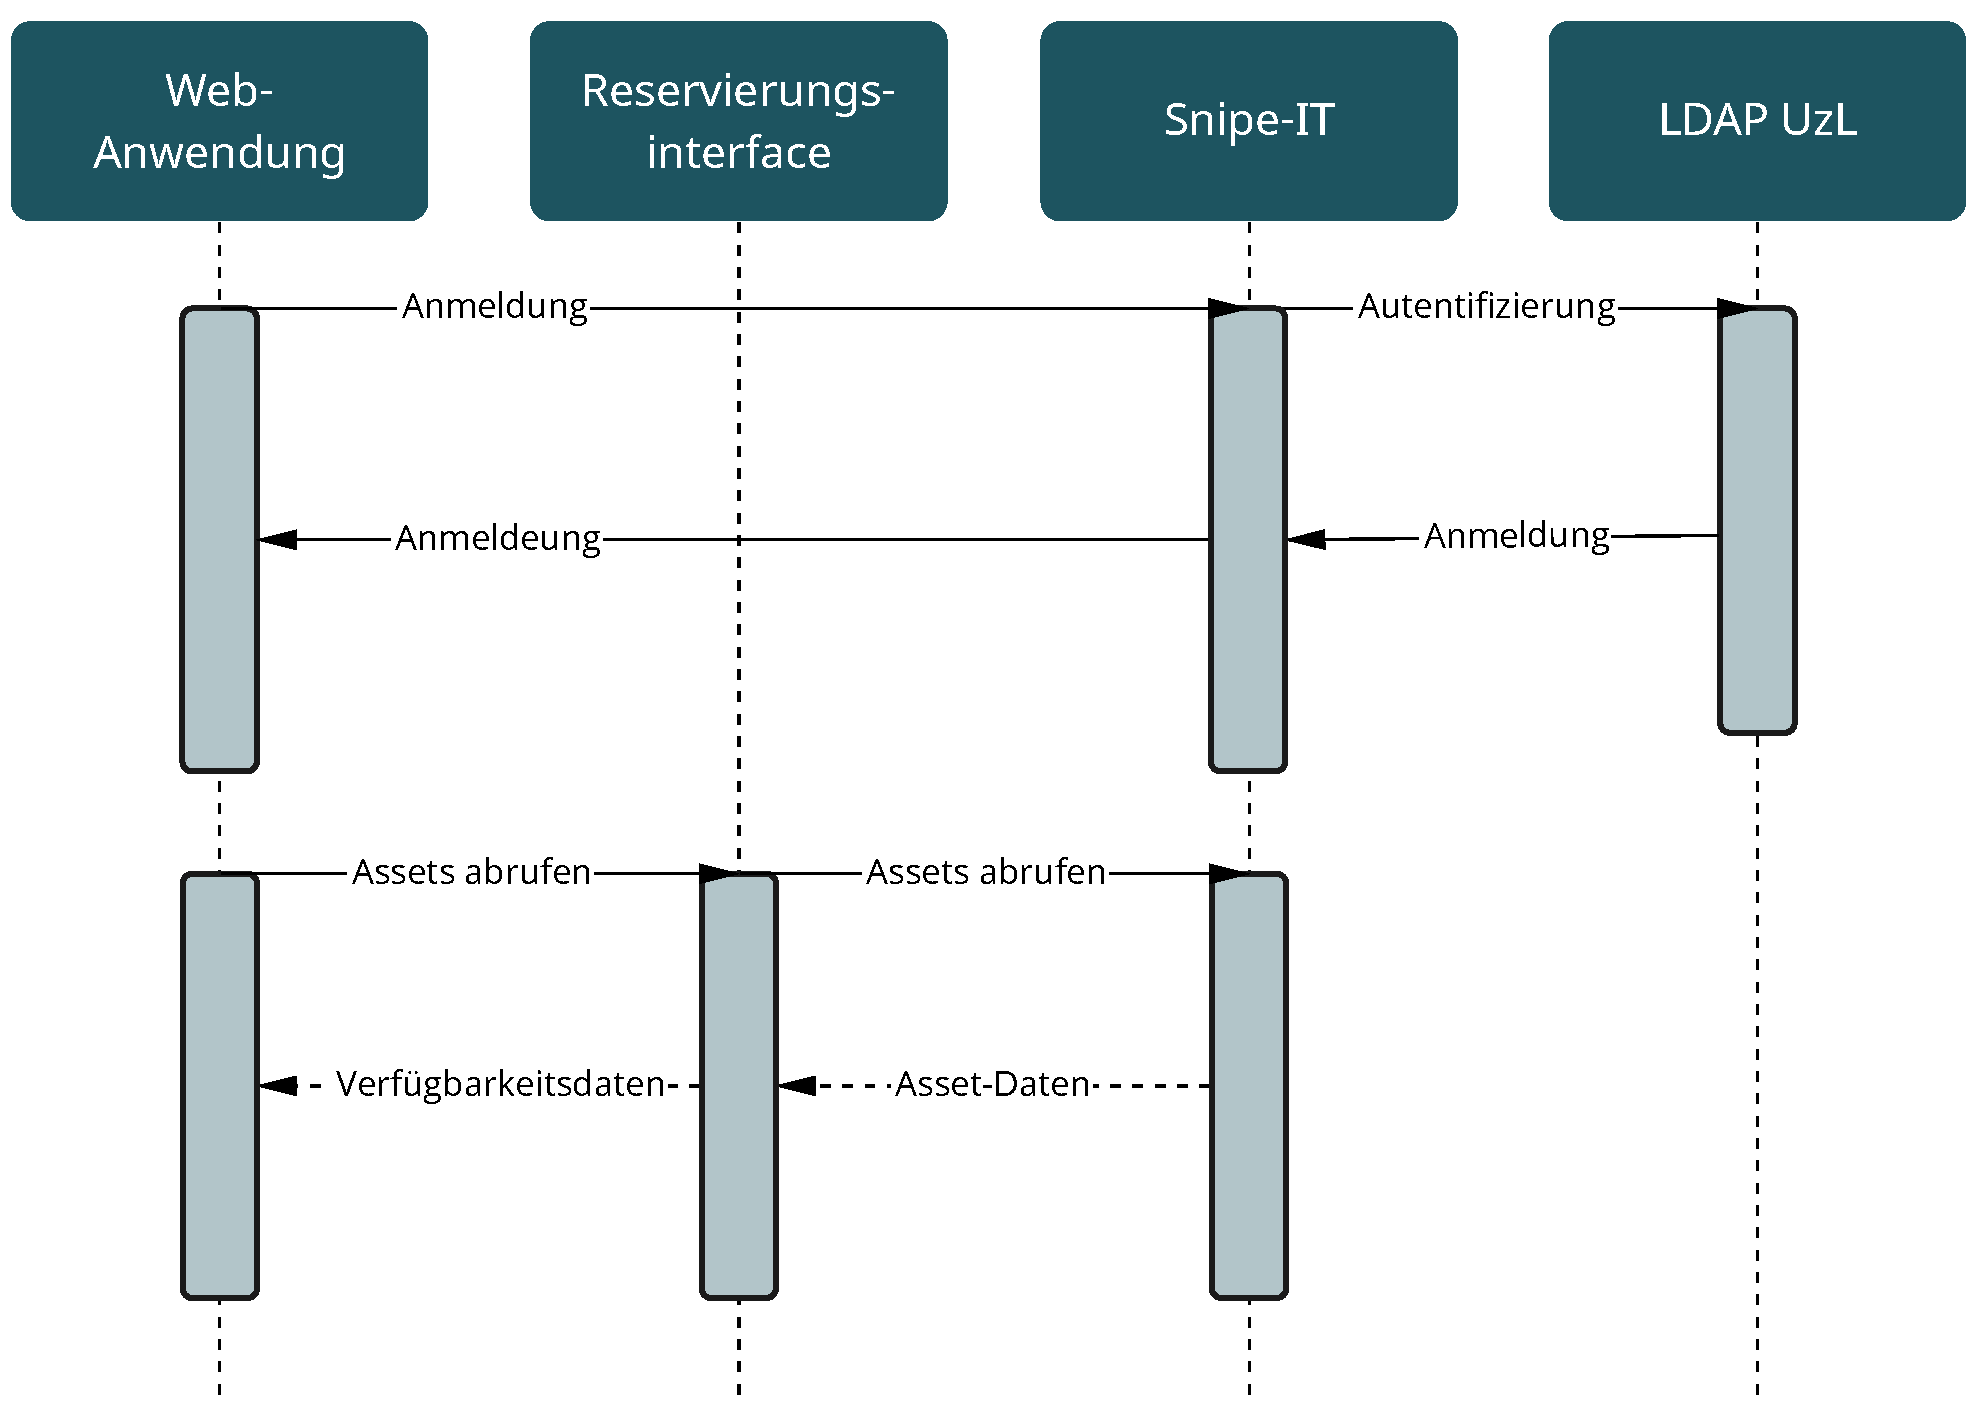
\includegraphics[scale=0.45]{Bilder/uml.pdf}
    \caption[UML-Sequenzdiagramm]{UML-Sequenzdiagramm}
    \label{fig:uml}
\end{figure}


